\documentclass[12pt, letterpaper]{article}

% Font
\usepackage[utf8]{inputenc}
\usepackage{MinionPro} 
\input{glyphtounicode}
\pdfgentounicode=1 
\usepackage{microtype}

% Format
\usepackage[letterpaper, margin = 1in]{geometry}
\setcounter{secnumdepth}{0}
\usepackage{titlesec}  
\titleformat*{\section}{\centering\normalfont\Large\bfseries}

% Links
\usepackage[colorlinks = true, linkcolor = black, urlcolor = black, citecolor = black]{hyperref} 

% Figures
\usepackage{graphicx}
\usepackage[labelfont = bf, font = small, labelsep = newline, singlelinecheck = false]{caption}
\renewcommand{\thefigure}{S\arabic{figure}}

% Tables
\usepackage{booktabs}
\usepackage{tabularx}

% Frontmatter
\title{ Supplemental Online Materials:\\\textit{Meta-Analysis of the `Ironic' Effects of Intergroup Contact} }
\author{  }

\begin{document}

\maketitle

\hypertarget{deviations}{%
\subsection{Deviations}\label{deviations}}

We preregistered the eligibility criteria, search strategy, study
selection, data collection, and preregistered analyses. Some aspects of
the preregistered protocol proved unrealistic, impractical, or
underspecified. Therefore, we deviated from the protocol in the
following ways:

\begin{enumerate}
\def\labelenumi{\arabic{enumi}.}
\item
  We preregistered that we would update our search every four months
  until we would submit the manuscript. This proved unrealistic as the
  study selection and data collection process for the new studies took
  almost as long. Instead, we concluded our search of electronic
  databases on April 1, 2020---that is, before we started analyzing and
  documenting our findings.
\item
  We preregistered that we would randomly select 100 records to be
  screened by both coders to calculate inter-rater agreement. We did not
  specify, however, what we would do if inter-rater agreement was less
  than acceptable. We decided to refine our coding strategy over three
  samples of 100 records until we achieved acceptable agreement.
\item
  We preregistered that we would use \emph{Google Scholar} to find
  records citing eligible studies. This proved impractical as
  \emph{Google Scholar} does not facilitate the electronic export of
  citing records. Instead, we used the \emph{Scopus} citation database.
\item
  We preregistered that we would attempt to contact the authors of all
  papers with missing effect sizes. Instead, we decided to not contact
  authors for studies published before 2000 as we considered it unlikely
  that the authors still had access to the data.
\item
  We preregistered that we would use a Bayesian two-level random-effects
  meta-analysis model, described in the main text, for all preregistered
  analyses. For the association between policy support and collective
  action, however, we had only few studies and found that the two-level
  model did not result in a reliable posterior distribution (as
  indicated by divergent transitions in the estimation algorithm).
  Instead, we used a Bayesian one-level random-effects model to estimate
  that association.
\end{enumerate}

\hypertarget{search-strategy}{%
\subsection{Search Strategy}\label{search-strategy}}

We used similar non-exclusive search terms for all electronic databases:

\begin{enumerate}
\def\labelenumi{\arabic{enumi}.}
\item
  (contact OR friendship) AND (``perceived discrimination'' OR
  ``perceived *advantage'' OR ``relative deprivation'' OR ``group
  discrimination'' OR ``personal discrimination'' OR ``group
  deprivation'' OR ``perception* of discrimination'' OR ``perception* of
  group discrimination'' OR ``perception* of personal discrimination''
  OR ``rac* discrimination'')
\item
  *group AND (contact OR friendship) AND (``collective action'' OR
  protest OR ``collective behavio*r'' OR ``political behavio*r'' OR
  ``social change'' OR ``social justice'')
\item
  *group AND (contact OR friendship) AND (policy OR policies OR
  ``affirmative action'' OR (politi* W/15 attitude*) OR (politi* W/15
  preferenc*)) AND (redistribut* OR reparati* OR inequalit* OR equalit*
  OR injustice* OR justice* OR disadvantage* OR advantage* OR minorit*
  OR majorit*)
\end{enumerate}

\noindent We sent a call for unpublished research to the mailing lists
of the \emph{European Association of Social Psychology}, the
\emph{Society for Personality and Social Psychology}, the
\emph{International Society of Political Psychology}, the \emph{Society
for the Psychological Study of Social Issues}, and the \emph{Society of
Australasian Social Psychologists}.

\hypertarget{robustness-checks}{%
\subsection{Robustness Checks}\label{robustness-checks}}

As preregistered, we conducted two kinds of robustness checks. First, we
assessed to what extent our findings were sensitive to choosing
narrower, \(\mu \sim \text{Normal}(0, 0.1)\), or wider,
\(\mu \sim \text{Normal}(0, 1)\), prior distributions. Choosing narrower
or wider prior distribution did not affect mean effect size estimates
for perceived injustice (\(\Delta r = -.00, [-.05, .04]\) and
\(\Delta r = .00, [-.05, .05]\)), collective action
(\(\Delta r = -.01, [-.11, .09]\) and \(\Delta r = .00, [-.11, .10]\)),
and policy support (\(\Delta r = -.01, [-.10, .08]\) and
\(\Delta r = .00, [-.09, .10]\)). Second, we assessed to what extent our
findings were sensitive to including or excluding influential studies by
repeating the preregistered analyses \(J\) times while leaving out one
of \(J\) studies each time and by calculating the mean absolute
difference (\emph{MAD}) for the estimated mean effect size across
left-out studies. For perceived injustice
(\(\textit{MAD} = .02, [.01, .04]\)), collective action
(\(\textit{MAD} = .04, [.02, .09]\)), and policy support
(\(\textit{MAD} = .03, [.02, .08]\)), the \emph{MAD} was small. Leaving
out the most influential study, for example, did not change estimates of
the mean effect size for the three outcomes
(\(\Delta r = .01, [-.04, .05]\); \(\Delta r = .02, [-.08, .12]\);
\(\Delta r = -.02, [-.11, .07]\)). Together, these analyses showed that
our findings were robust to choosing different prior distributions and
to excluding influential studies.

\hypertarget{moderator-analyses}{%
\subsection{Moderator Analyses}\label{moderator-analyses}}

First, we ran a series of Bayesian random-effects meta-regression models
to estimate how much of the between-samples heterogeneity was explained
by specific categorical moderator variables
(\texttt{run\_moderator\_analyses.R}). Figures S1 and S2 show the
results for collective action and policy support. Comparisons were
inconclusive because we had an insufficient number of effect sizes per
category. We ran another three random-effects meta-regression models
with Muthukrishna et al.'s (2020) measure of cultural distance, where
available, as a continuous moderator variable. Because cultural distance
was a country-level moderator variable, we used two-level random-effects
models in which we estimated country-specific deviations from the mean
effect size as well as sample-specific deviations from the
country-specific effect size. Figure 5 (in the main text) show the
inconclusive results for all three outcomes.

Second, we used meta-regression trees to discover interactions between
moderator variables that best explained heterogeneity in effect sizes
(Li et al., 2017, 2020). As recommended, we ran random-effects
meta-regression tree analyses using the look-ahead strategy (Li et al.,
2020). We set the pruning parameter to \(c = 0\) because, for this
analysis, we prioritized exploration over error control
(\texttt{run\_exploratory\_moderator\_analyses.R}). For both collective
action and policy support, the algorithm found that no moderator or
interaction of moderators explained between-samples heterogeneity. This
result is not surprising, however, as both analyses used fewer than 40
effect sizes, the minimum number required for the algorithm to perform
well in detecting even simple interaction effects (Li et al., 2017). As
all moderator analyses were inconclusive for collective action and
policy support, we only report results for perceived injustice in the
main text.

\begin{figure*}
\centering
\caption{Estimated effect sizes for the association between intergroup contact and collective action as a function of various categorical moderator variables}
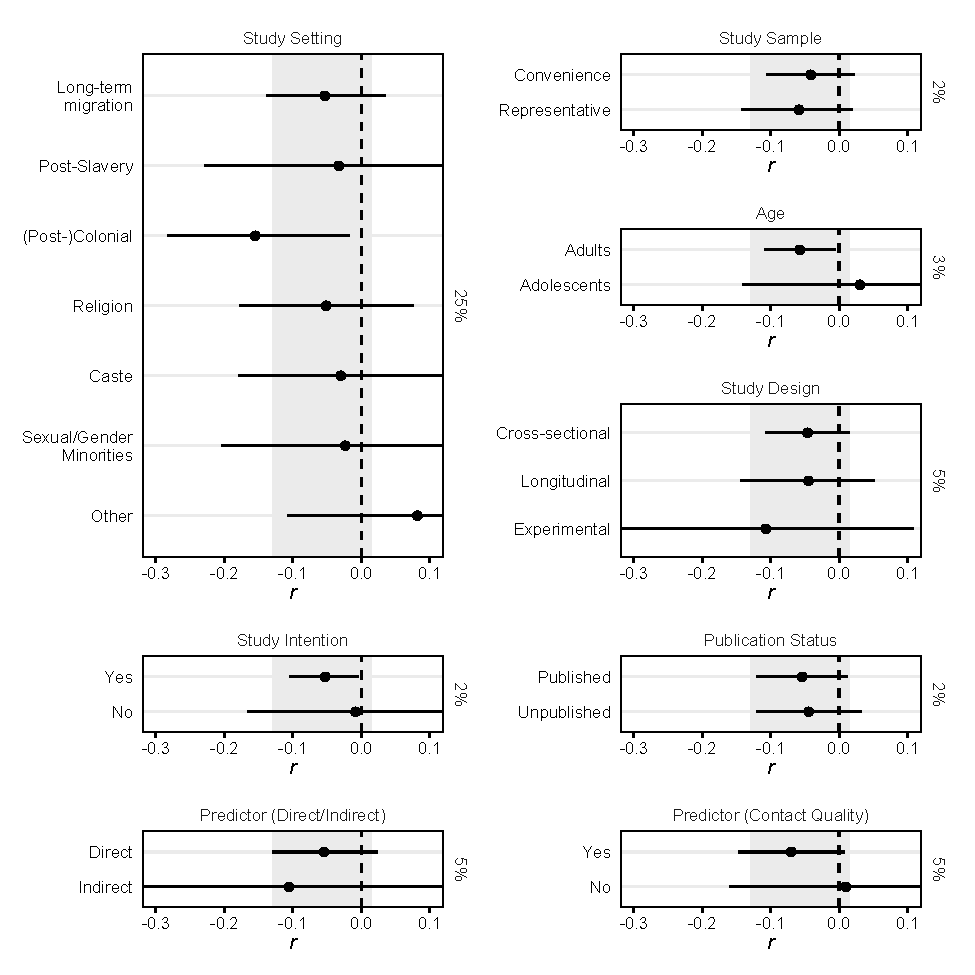
\includegraphics[scale=1]{../figures/figure-s1}
\caption*{\textit{Note.} Intervals enclose the 95\% most plausible estimates of the category-specific effect size. Shaded ribbons enclose the 95\% most plausible estimates of the mean effect size from the main analyses. Percentages indicate the estimated between-sample variance explained by each moderator variable.}
\label{fig:s1}
\end{figure*}

\begin{figure*}
\centering
\caption{Estimated effect sizes for the association between intergroup contact and policy support as a function of various categorical moderator variables}
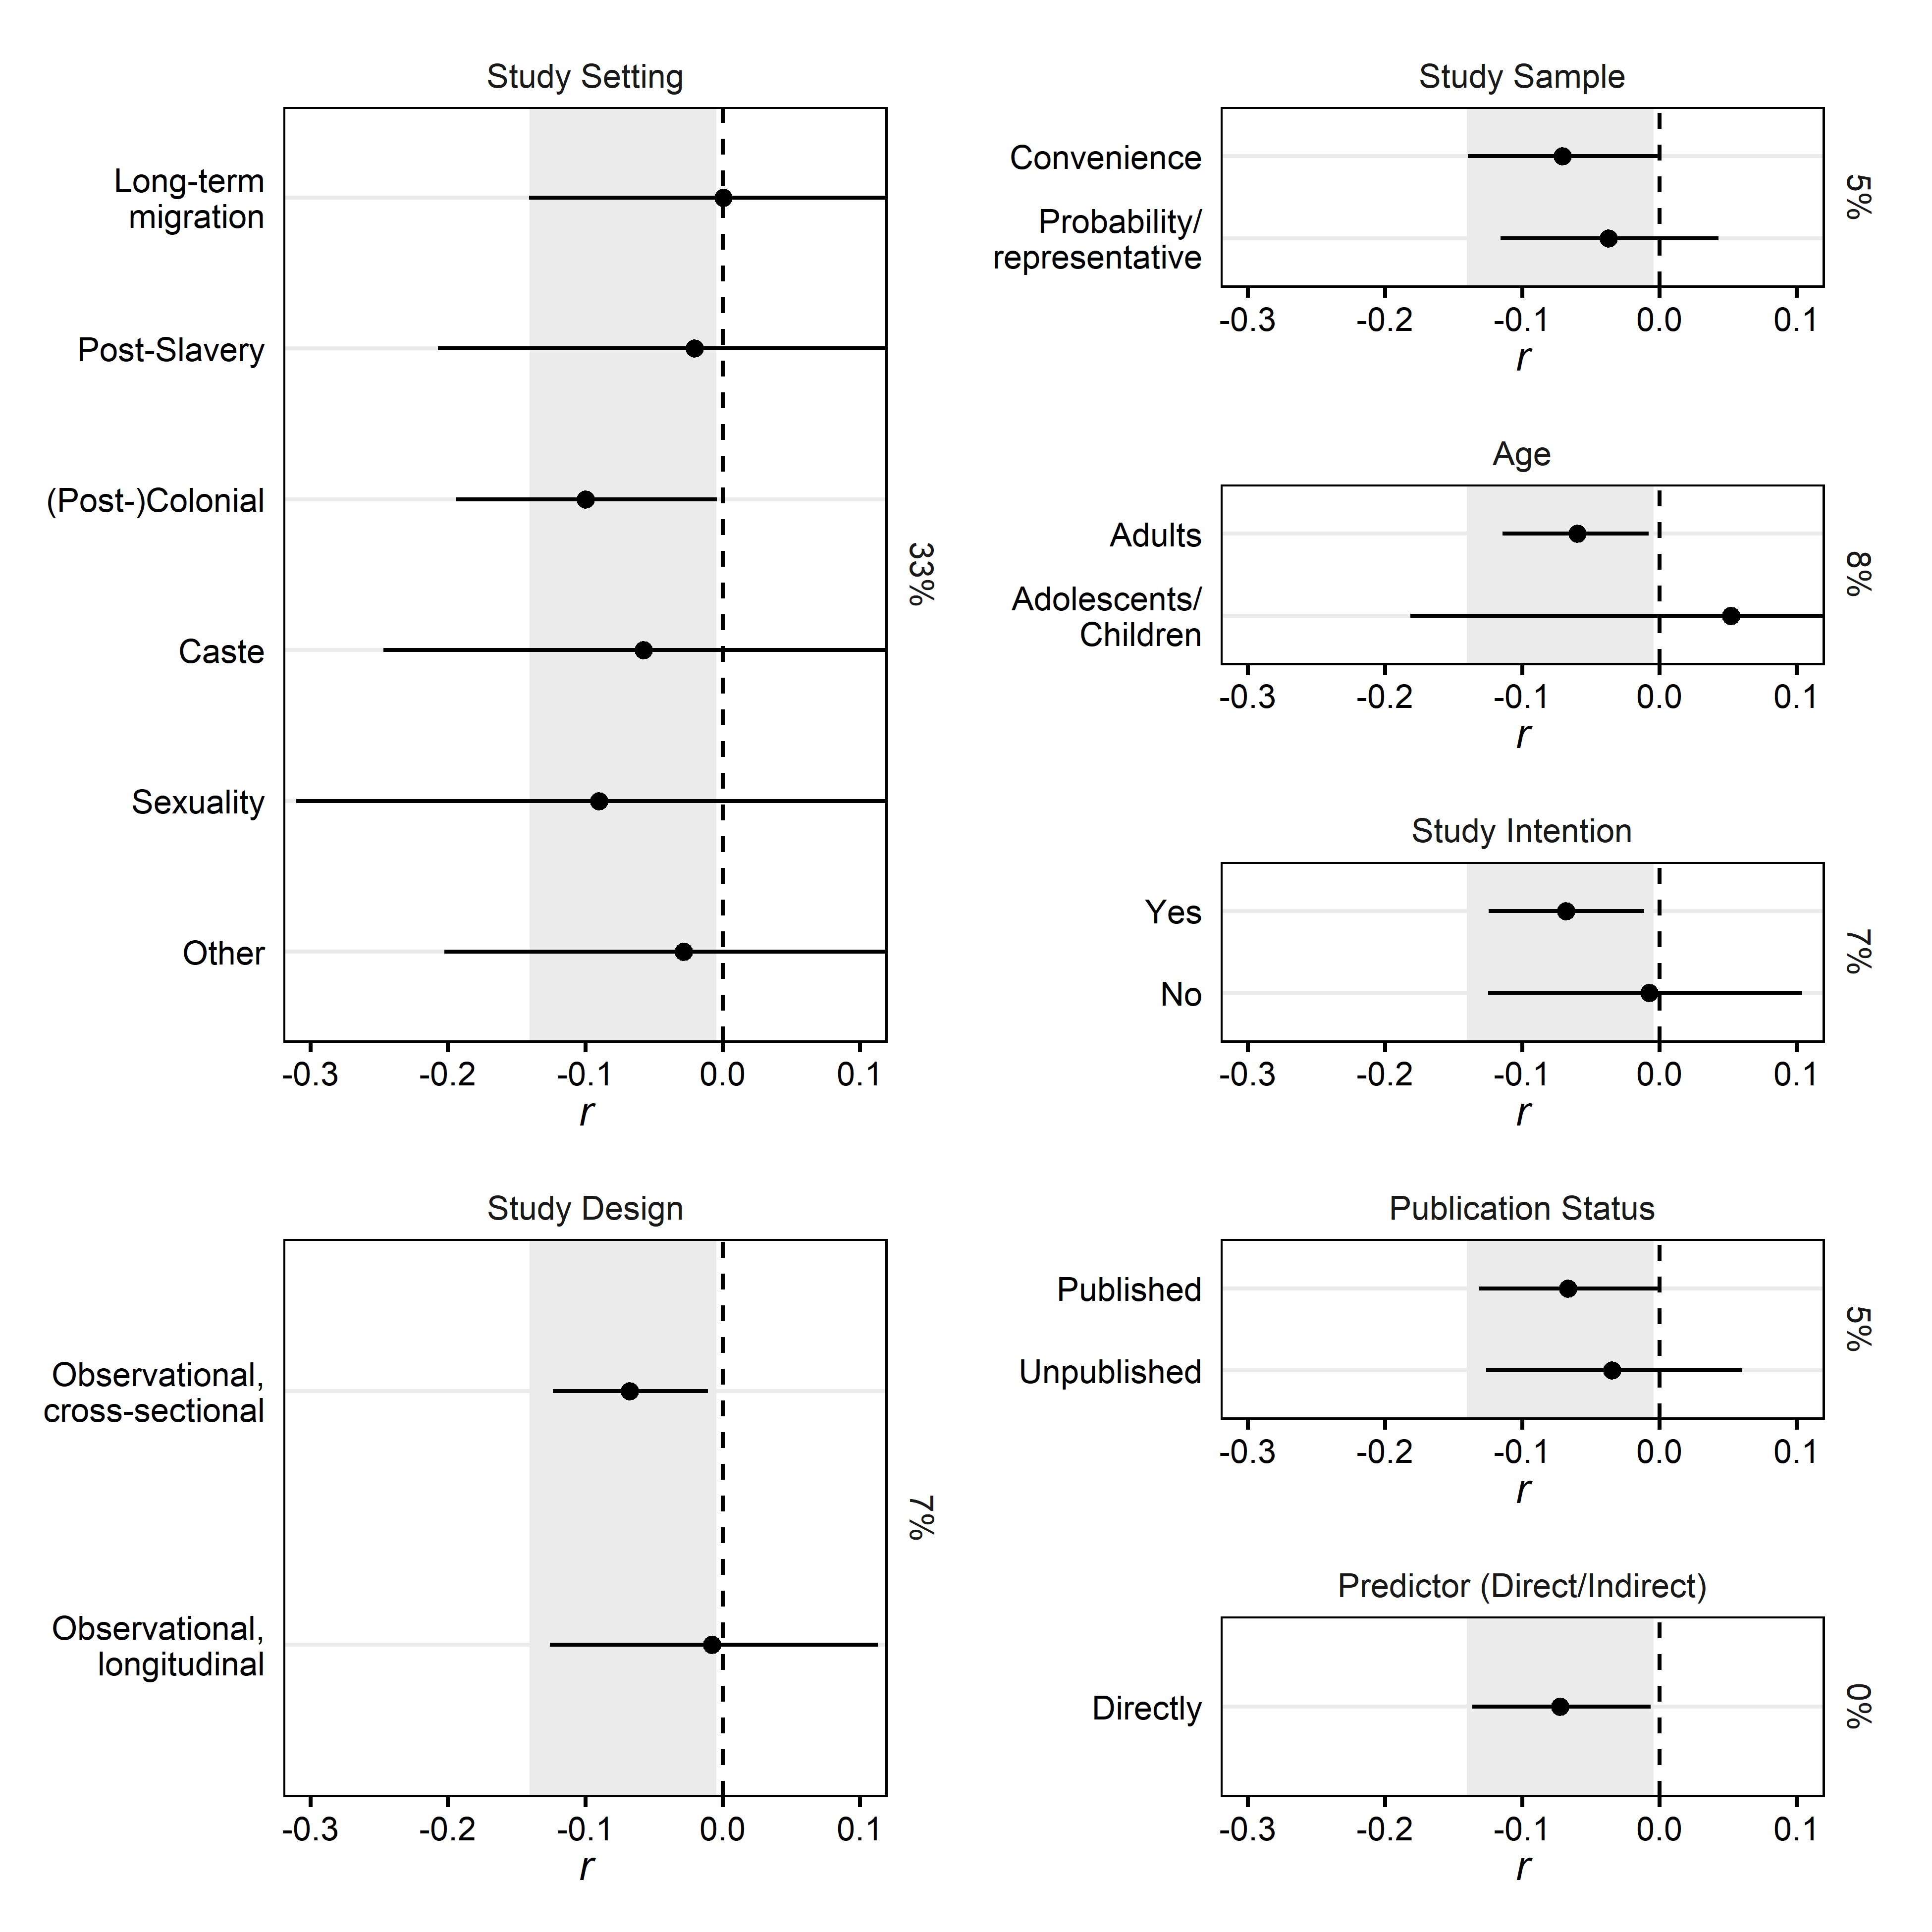
\includegraphics[scale=1]{../figures/figure-s2}
\caption*{\textit{Note.} Intervals enclose the 95\% most plausible estimates of the category-specific effect size. Shaded ribbons enclose the 95\% most plausible estimates of the mean effect size from the main analyses. Percentages indicate the estimated between-sample variance explained by each moderator variable.}
\label{fig:s2}
\end{figure*}

\hypertarget{references}{%
\section{References}\label{references}}

\begingroup

\noindent \setlength{\parindent}{-0.5in} \setlength{\leftskip}{0.5in}

\hypertarget{refs}{}
\leavevmode\hypertarget{ref-li_meta-cart_2017}{}%
Li, X., Dusseldorp, E., \& Meulman, J. J. (2017). Meta-CART: A tool to
identify interactions between moderators in meta-analysis. \emph{British
Journal of Mathematical and Statistical Psychology}, \emph{70}(1),
118--136. \url{https://doi.org/10.1111/bmsp.12088}

\leavevmode\hypertarget{ref-li_multiple_2020}{}%
Li, X., Dusseldorp, E., Su, X., \& Meulman, J. J. (2020). Multiple
moderator meta-analysis using the R-package Meta-CART. \emph{Behavior
Research Methods}, \emph{52}(6), 2657--2673.
\url{https://doi.org/10.3758/s13428-020-01360-0}

\leavevmode\hypertarget{ref-muthukrishna_beyond_2020}{}%
Muthukrishna, M., Bell, A. V., Henrich, J., Curtin, C. M., Gedranovich,
A., McInerney, J., \& Thue, B. (2020). Beyond western, educated,
industrial, rich, and democratic (WEIRD) psychology: Measuring and
mapping scales of cultural and psychological distance.
\emph{Psychological Science}, \emph{31}(6), 678--701.
\url{https://doi.org/10.1177/0956797620916782}

\endgroup

\end{document}